\documentclass[a4paper]{jpconf}
\usepackage{graphicx}
\usepackage{float}
\usepackage[export]{adjustbox}
\usepackage{subfig}
\renewcommand{\baselinestretch}{} 
%======================================================================================================================
% DELETE FROM RELEASE:
%======================================================================================================================
\usepackage{hyperref}
\hypersetup{
  colorlinks = true,
  urlcolor = blue,
  pdfauthor = {Alexander Mazurov},
  pdfkeywords = {scientific computing, system and distributing programming},
  pdftitle = {Advanced Modular Software Performance Monitoring},
  pdfsubject = {Advanced Modular Software Performance Monitoring},
  pdfpagemode = UseNone
}

\usepackage{lineno}
% Customize page headers
\usepackage{fancyhdr}
\setlength{\headheight}{15.2pt}
\pagestyle{fancyplain}
\renewcommand{\baselinestretch}{2.0}
 
\fancyhf{}
\lhead{\fancyplain{}{{\bf Version 1.0} (\today)}}
\rhead{\fancyplain{}{\href{https://github.com/mazurov/chep2016/compare/v1.9...v1.10}{https://github.com/mazurov/chep2012/compare/v1.9...v1.10}}}

\linenumbers
%======================================================================================================================
\captionsetup[subfigure]{subrefformat=simple,labelformat=simple,listofformat=subsimple}
\renewcommand\thesubfigure{(\alph{subfigure})}
%======================================================================================================================


\begin{document}
\title{Microservices for systematic profiling and monitoring of the refactoring process at the LHCb experiment}
\author{A Mazurov\ad{1} and B Couturier\ad{2}}
%======================================================================================================================
% DELETE FROM RELEASE:
%======================================================================================================================
\thispagestyle{fancy}
%======================================================================================================================
\address{\ad{1} University of Birmingham, Birmingham, United Kingdom}
\address{\ad{2} CERN, European Organization for Nuclear Research, Geneva, Switzerland}


\ead{alexander.mazurov@cern.ch}


\newcommand\iamp{{Intel\textsuperscript{\textregistered} VTune\texttrademark Amplifier XE} }
\newcommand\amp{{VTune\texttrademark Amplifier XE} }
\newcommand\intel{{Intel\textsuperscript{\textregistered}} }
\newcommand\google{{Google\textsuperscript{\textregistered} }}
\newcommand\docker{\textit{Docker} }
\newcommand\compose{\textit{Compose} }
\newcommand\composes{\textit{Compose's} }

\begin{abstract}
Any time you modify an implementation within a program, change compiler version
or operating system, you should also do regression testing. You can do
regression testing by rerunning existing tests against the changes to determine
whether this breaks anything that worked prior to the change and by writing new
tests where necessary. At LHCb we have a huge codebase which is maintained by
many people and can be run within different setups. Such situation leads to the
crucial necessity to guide refactoring with a central profiling system that
helps to run tests and find the impact of changes.

In our work we present a software architecture and tools for running a profiling
system. This system is responsible for systematically running regression tests,
collecting and comparing results of these tests, so changes between different
setups can be observed and reported. The main feature of our solution is that it
is based on a microservices architecture. Microservices break a large project
into loosely coupled modules, which communicate with each other through simple
APIs. Such modular architectural style helps us to avoid general pitfalls of
monolithic architectures such as hard to understand and maintaining of a large
codebase and ineffective scalability. Our solution also allows to escape a
complexity of microservices deployment process by using software containers and
services management tools. Containers and service managers let us quickly deploy
linked modules in development, production or in any other environments. Most of
the developed modules are generic which means that the proposed architecture and
tools can be used not only in LHCb but adopted for other experiments and
companies. \end{abstract}

\section{Introduction}

In LHCb, as in all High Energy Physics (HEP) experiments, complex software is
used to process the data recorded by the detectors. Whenever developers change
or modify their software, even a small tweak can have unexpected
consequences. Regression and performance testing is testing existing software
applications to make sure that a change don't broke or degradate any existing
functionality. The purpose of these tests is to catch issues that may have been
introduced into a new build, and to ensure that previously eradicated issues
continue to stay fixed. By re-running testing scenarios that were originally
scripted when known problems were first fixed, you can make sure that any new
changes to an application haven't resulted in a regression, or caused components
that formerly worked to fail. Such tests can be performed manually on small
projects, but in the HEP software repeating a suite of tests each time an update
is made is too time-consuming and complicated to consider, so an automated
testing tool is required. 

The LHCb Performance and Regression~(LHCbPR)~\cite{lhcbpr}  project is a key
component in the LHCb Software~\cite{lhcbsoft} development which provides
support to conduct systematic profiling and allows comparing the results of
performance and regression tests run on the LHCb applications. In this paper we
introduce a new architecture and implementation of LHCbPR system which allows to
avoid some major pitfalls of the previous version~\cite{lhcbpr}.

The Section~\ref{sec:arch} gives a brief overview of the previous LHCbPR version,
its advantages and disadvantages, following by the description of the
new architecture. In the Section~\ref{sec:impl} the implementation details are outlined.
Real examples are shown in the forth section.

\section{LHCbPR Software Architecture}\label{sec:arch}

Figure~\ref{fig01} presents a general sequence diagram of interaction between
the tests running service, LHCbPR  and users. The
test service requests from LHCbPR information on how to run tests, run tests
and then save results back to LHCbPR. Users have an ability to retrieve and
analyse these tests' results.

\begin{figure}[H]
\begin{minipage}{\textwidth}
\centering
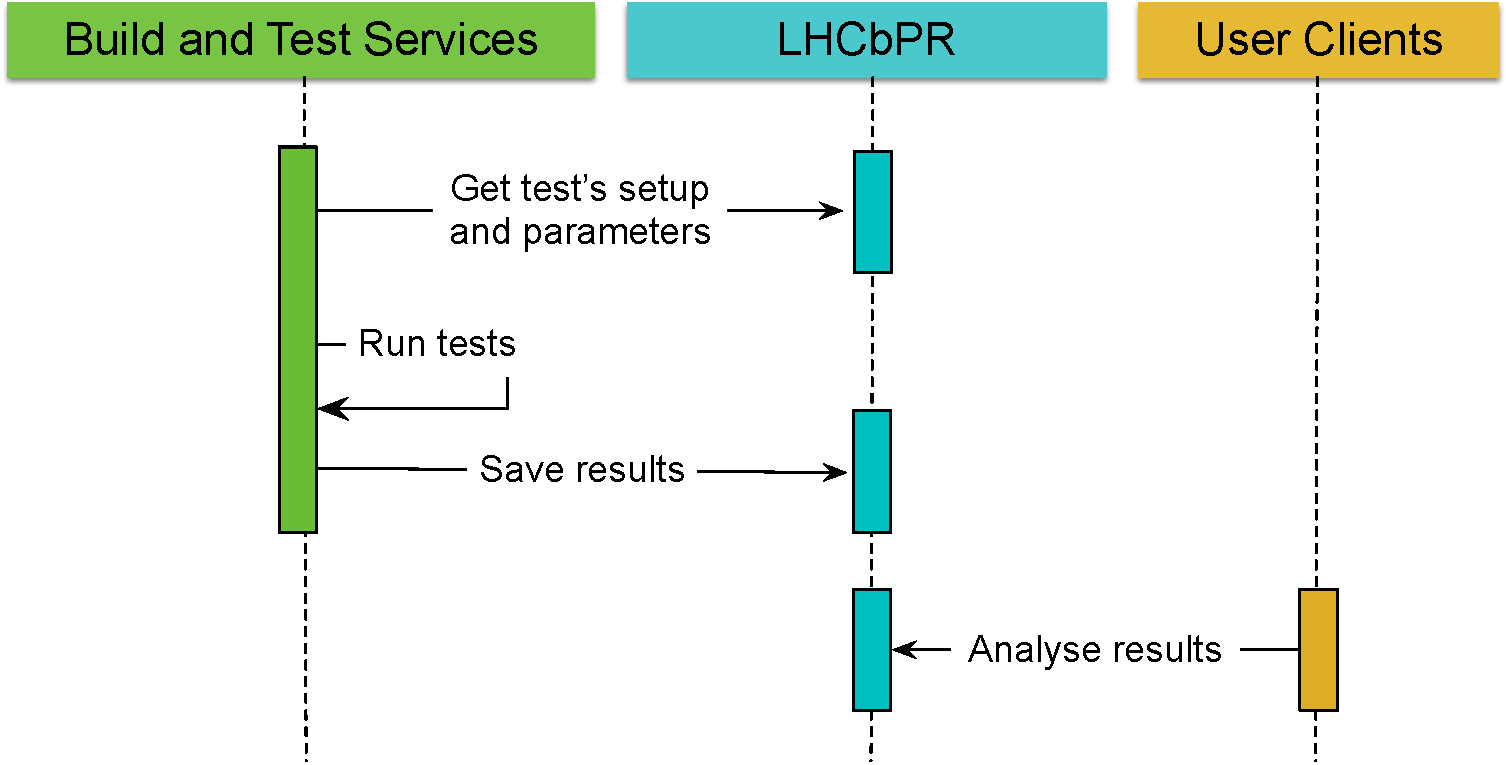
\includegraphics[width=0.8\textwidth]{figs/lhcbpr-general.pdf}
\caption{\label{fig01} General sequence diagram of interaction between test
running services, LHCbPR and users}
\end{minipage}
\end{figure}

% https://impact.hackpad.com/Advantages-and-Disadvantages-of-a-Monolith-Application-ZlrQRl3LHCg
% http://microservices.io/patterns/monolithic.html
\subsection{Monolithic architecture}
The first version of the LHCbPR had a monolithic architecture, in which all
functionality is integrated into one application. All components of
such application are stored in one codebase that leads to the common inherent
issues like:
\begin{itemize}
\item The application can be difficult to understand and modify. That
intimidates new developers and slow down the development process.
\item There are usually no hard boundaries between components and that
boundaries are easy to break.
\item Continuous deployment is difficult since in order to update one component
you have to redeploy the entire application. This is especially an issue in
components that requires rapid and frequent redeployment, like user interfaces.
\item A monolithic application forces you to be coupled to the certain
technology stack. That leads to the situation where, for example, can be
difficult to adopt a newer technology stack.
\end{itemize}

The monolithic architecture was chosen initially since it has benefits at the
prototyping stage of the software products:
\begin{itemize}
\item Simple to develop a small application since you are working with one codebase
and all developers uses the same technology stack.  
\item Simple to deploy application since you usually have to run the application in the same
runtime and environment.
\item Simple to scale --- you can run multiply copies of the application behind a
load balancer.
\end{itemize}

But the advantages of such architecture works only for small applications,
usually at the time when you only start to develop it. In the growing
monolithic application the disadvantages become more annoying and slow down the
development process. One of the solution is to use the microservices architecture.  

\subsection{Microservices Architecture}

In opposite to the monolithic architecture, in the microservices architecture
applications are built from the smaller components, which, usually, are stored
in separate codebases and are independent from each other. In the new version of LHCbPR
components communicate through a simple Application Programming
Interfaces (APIs). Such component are commonly named microservices.

Microservices help to avoid general pitfalls of the monolithic architecture.
Smaller components easier to understand and modify. There are strict boundaries
between components and it is almost impossible to break one component by modifying
the other. Only changes of API can lead to some  disruptions.   

Solutions based on microservices have a number of drawbacks:
\begin{itemize}
\item Complexity of creating distributed system.
\begin{itemize}
\item We need to have a good coordination between component's teams. In 
the development process APIs can be modified which can lead to the rewriting of
some components' parts. 
\item In distributed systems we have to use the communication technologies that
usually not needed in monolithic applications. For example, microservices can be
run on different nodes and communicate with each other through synchronous HTTP
interface or through asynchronous messaging systems.  
\end{itemize}
\item Deployment complexity.  Each of the component can be run in  different
environments and use various technologies, which leads to additional efforts for
supporting and deploying such systems.
\end{itemize}

The next section shows details of the new LHCbPR implementation and outline how
major microservices pitfalls were solved.


\section{LHCbPR implementation}\label{sec:impl}

Figure~\ref{figLHCbPR2}  details the implementation of the new LHCbPR microservices
architecture. 

\begin{figure}[H]
\begin{minipage}{\textwidth}
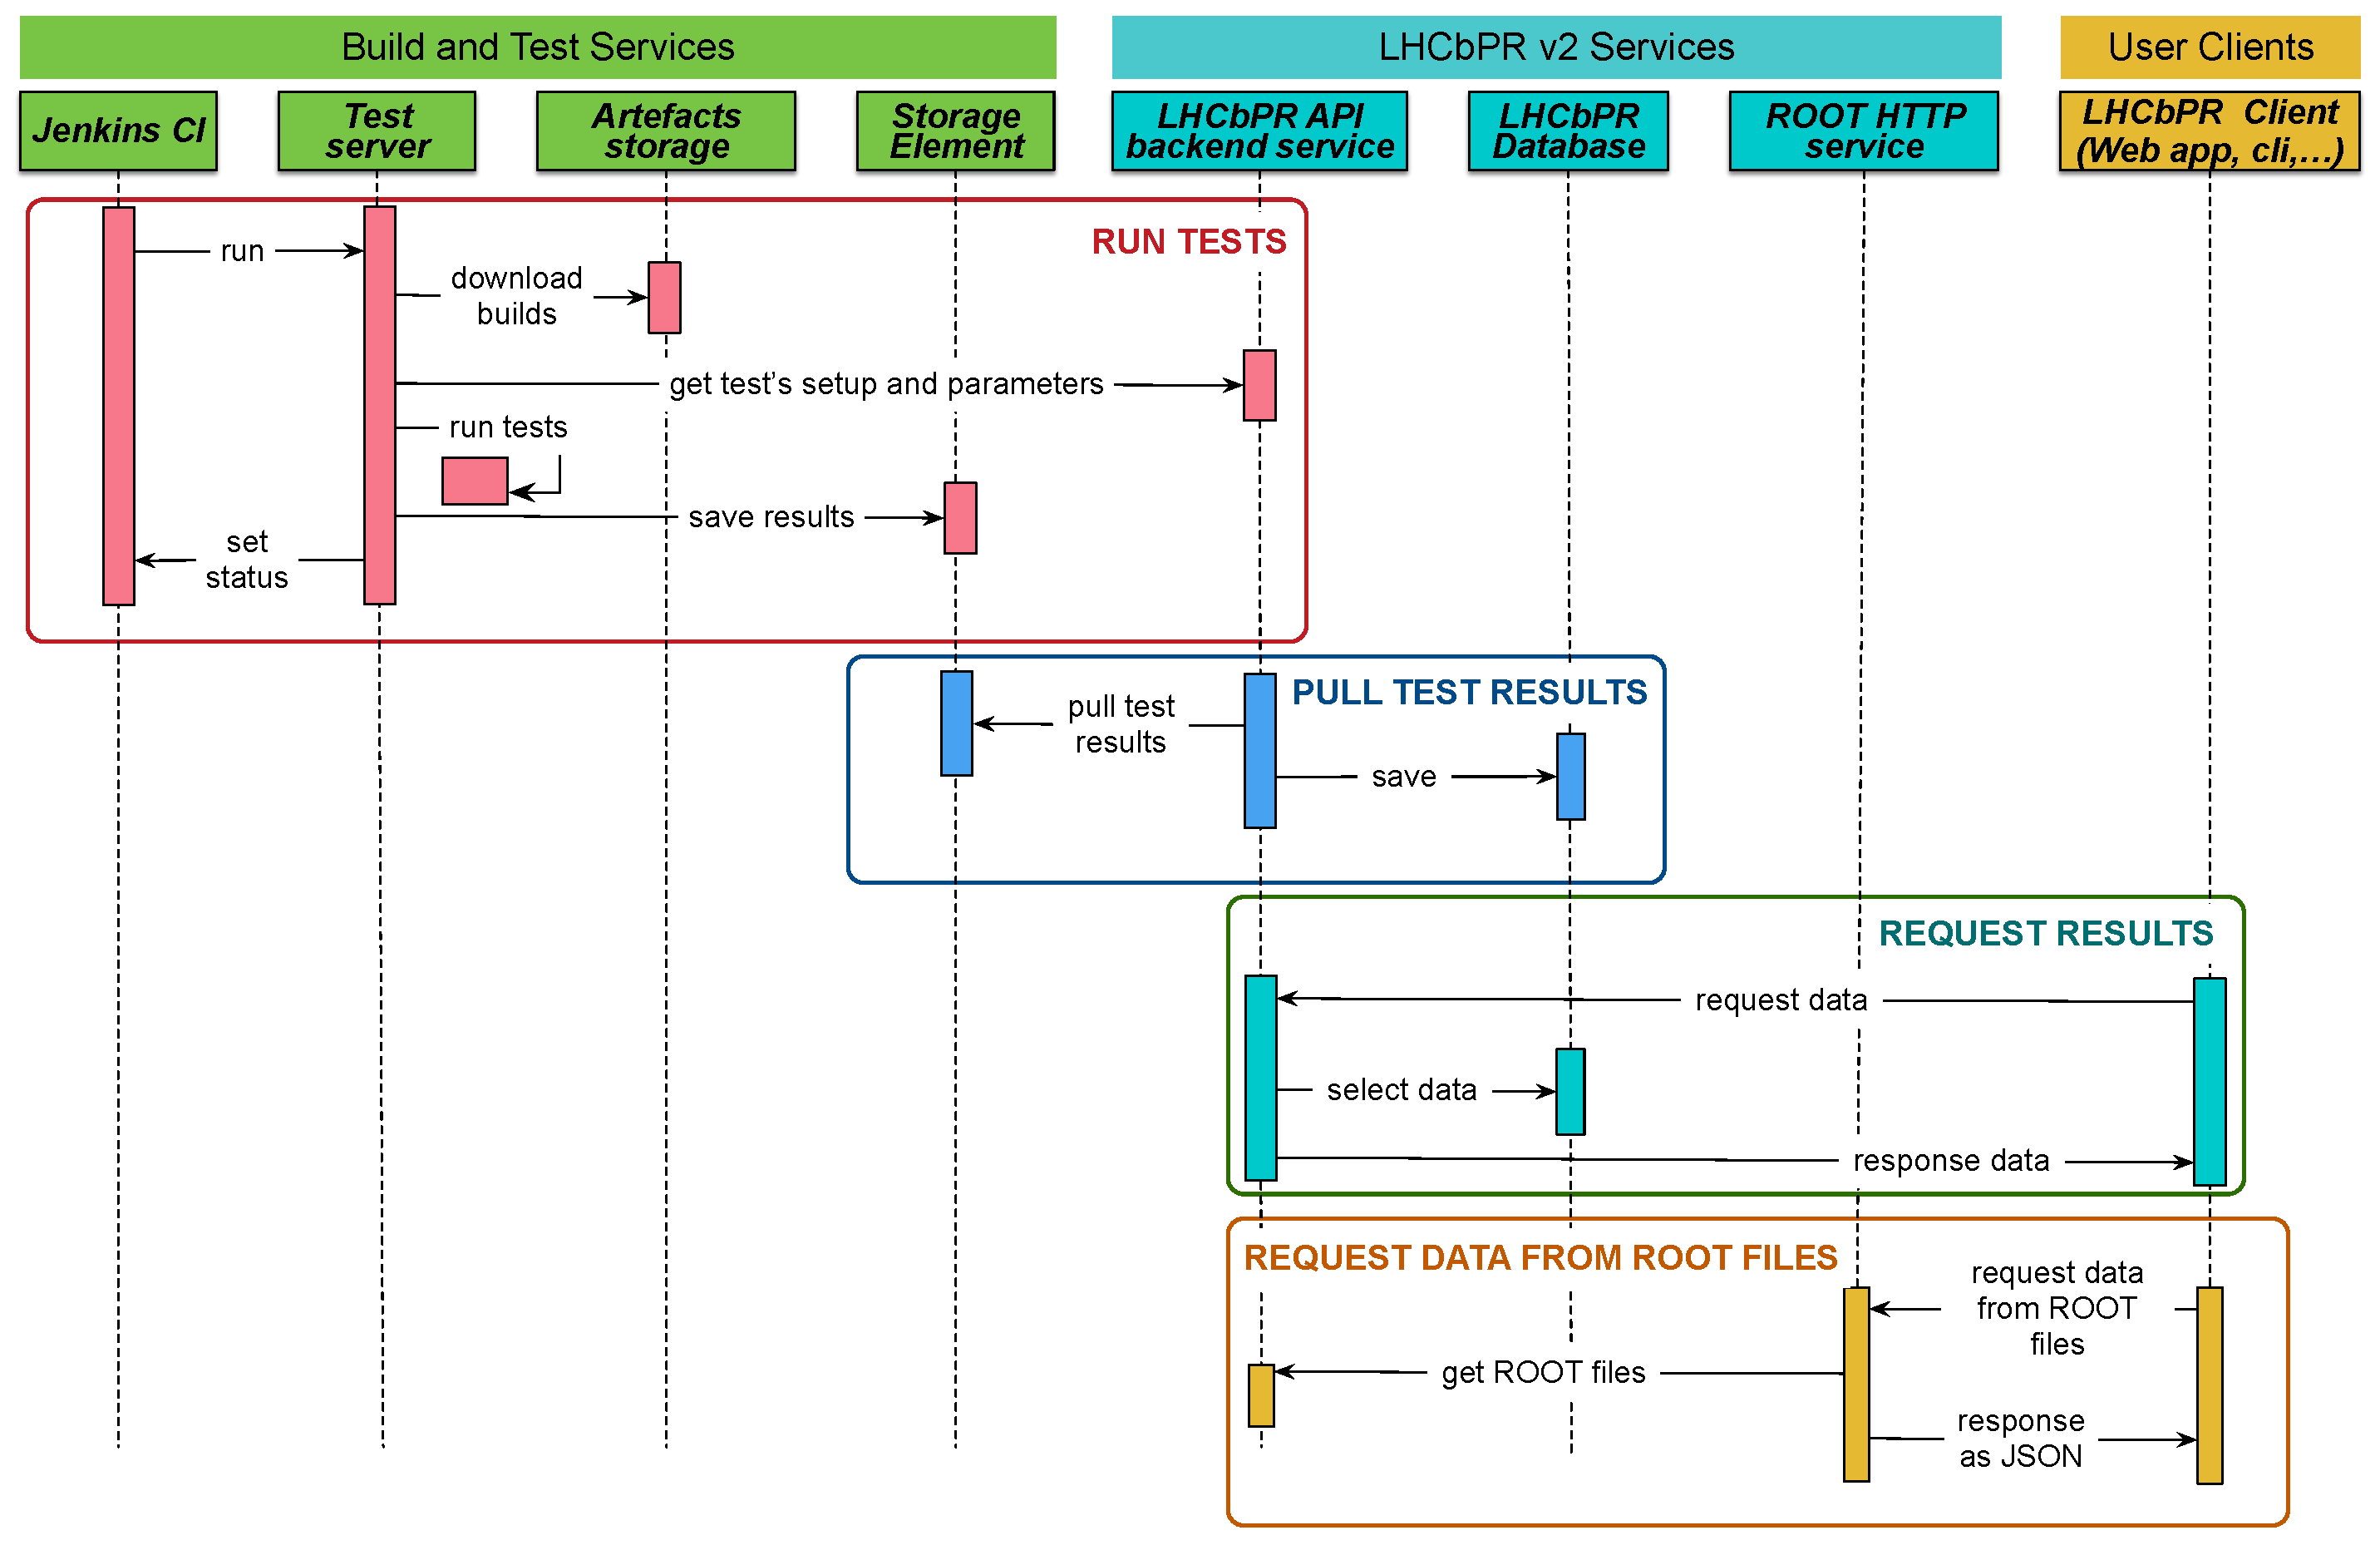
\includegraphics[width=\textwidth]{figs/LHCbPR2.pdf}
\caption{\label{figLHCbPR2} LHCbPR~v2. Sequence diagram of interaction between test
running services, LHCbPR's microservices and users.}
\end{minipage}
\end{figure}

The test service communicates with LHCbPR for the following purposes:
\begin{itemize}
\item \textbf{Retrieve test parameters}. The test manager configures schedule
for running tests. Each record of the schedule provides information about the
build environment: application under the test, name of the test, name of the
special software handler for test results postprocessing, operating system,
compiler version, machine architecture. At the scheduled time the test service
requests an additional information from LHCbPR application: the name of the
program for running the test, path to the test script. After the testing finish
the required  test results are saved to LHCbPR. All information about the tests
and its result are stored at MySQL database. The other components can access
database throw the LHCbPR API backend microservice. This service is the REST web
service that allows clients to retrieve and update information in database be making
HTTP requests. The advantage of the service is that it hides database
implementation --- clients can retrieve only information that the service provides
and could not directly access the database. Most of the changes in the database schema
or in the database engine are almost transparent for the service clients.

\item \textbf{Save test results}. Test results are packed by test service into
an archive file and uploaded to the network storage. LHCbPR backend service pull
the results into the database by executing the corresponding import script.
Results become immediately accessible throw the REST API.
\end{itemize}

\subsection{API  service}
The API service is open for any program that supports HTTP
requests. The common use of the service is to retrieve test results which are
provided in JSON. For example, the important part of the LHCbPR
infrastructure is a web application (Section~\ref{sec:webapp}), which allows users
to search and analyse results. This
application is build on top of two services: (1)~the LHCbPR API service
and (2)~LHCbPR ROOT service~(Section~\ref{sec:rootapp}). 


\subsection{ROOT service}\label{sec:rootapp}

In many tests that are used in HEP the output contains histograms and graphs.
One of the possible regression testing analysis is to compare histograms. Such
comparison can be done by presenting histograms' ratio or by evaluating the
Kolmogorov probability. In LHCbPR we developed a web microservice that can
convert almost any ROOT object into JSON and output histograms comparison
results. This functionality is based on the TBufferJSON class in ROOT. Any user
client can retrieve results by making simple http requests and analyse the
output without installing ROOT.


\subsection{Web application}\label{sec:webapp}

The regression tests does not make sense if there are no tool for analyzing the
results. For that reason it was created a web frontend that uses the API and
ROOT services described above.

This frontend has the following functions:
\begin{itemize}
\item \textbf{Find test results} by their parameters like name, application,
platform. Figure~\subref*{fig:webapp:search} shows an example of the corresponding
interface.
\item \textbf{Compare and present the results} of the selected tests in the user-friendly interface.
\end{itemize}

The frontend is a single-page AngularJS~\cite{angular} web application that loads a single HTML page and
dynamically update that page as the user interacts with the application. We use
web server only for handling static pages and all operation with the related
microservices are done with AJAX requests.

The main part of the web application is an analysis module --- a set of
javascript code and HTML that is responsible for combining and presenting the
selected tests. Analysis modules works like plugins --- each module is stored in
the dedicated folder and not depends from the other modules. The application is
structured so people can work independently on modules. For the developers
convenience the main library contains a set of web components that implements
the functionality common for the most of the analysis modules. For example, the
common components are the form for searching test results and component for
displaying histograms retrieved from the ROOT service.

The application can have as many analysis modules as a number of tests or even
more. But it's not necessary to create analysis for each test beacause the
application includes generic modules that can handle results of the most of the
tests. For example, it includes a module that can plot trend analysis of any
numeric value that was probed in different versions of some application. Another
generic module can compare histograms from the any ROOT files provided in the
test results as it is shown at Figure~\subref*{fig:webapp:analyse}.


\begin{figure}[H]
\centering
\subfloat[Search tests' results. Search form (left) and search results table
(right).]{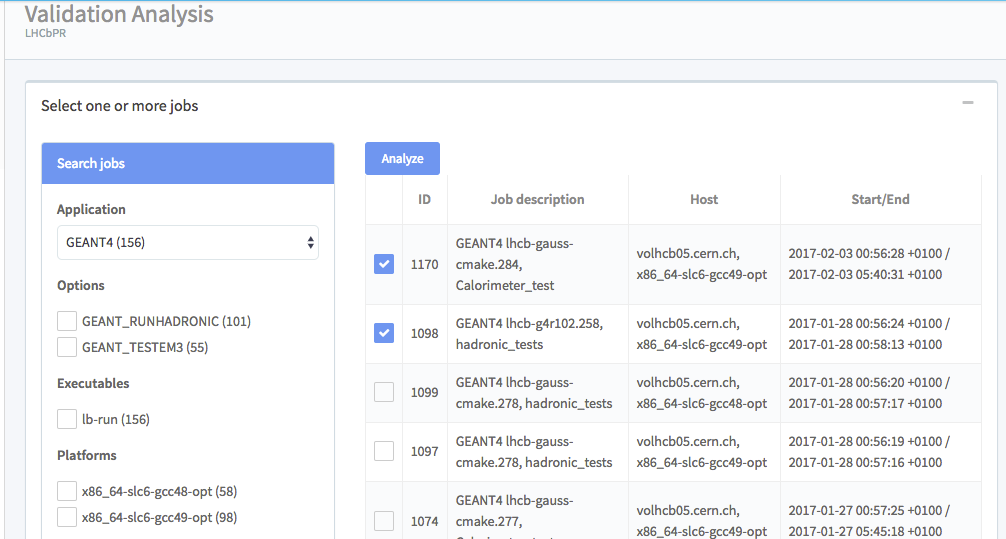
\includegraphics[width=0.6\textwidth,valign=t]{figs/webapp.png}\label{fig:webapp:search}}
\quad
\subfloat[Show difference of the histograms from the selected tests]{
  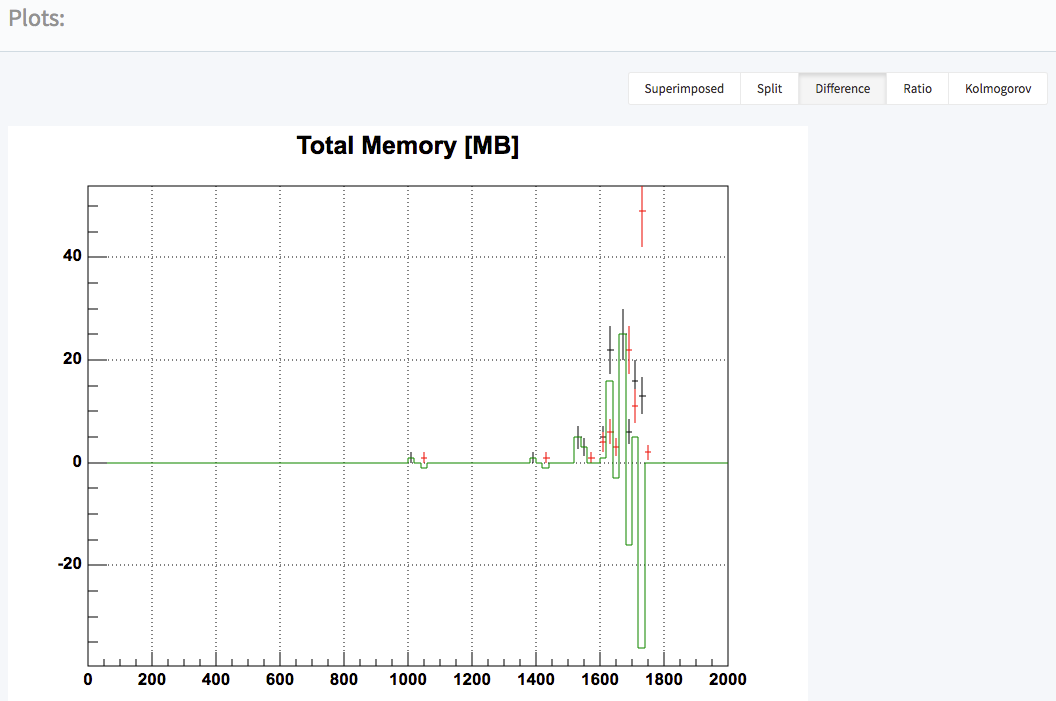
\includegraphics[width=0.35\textwidth,valign=t]{figs/webappplots.png}
  \vphantom{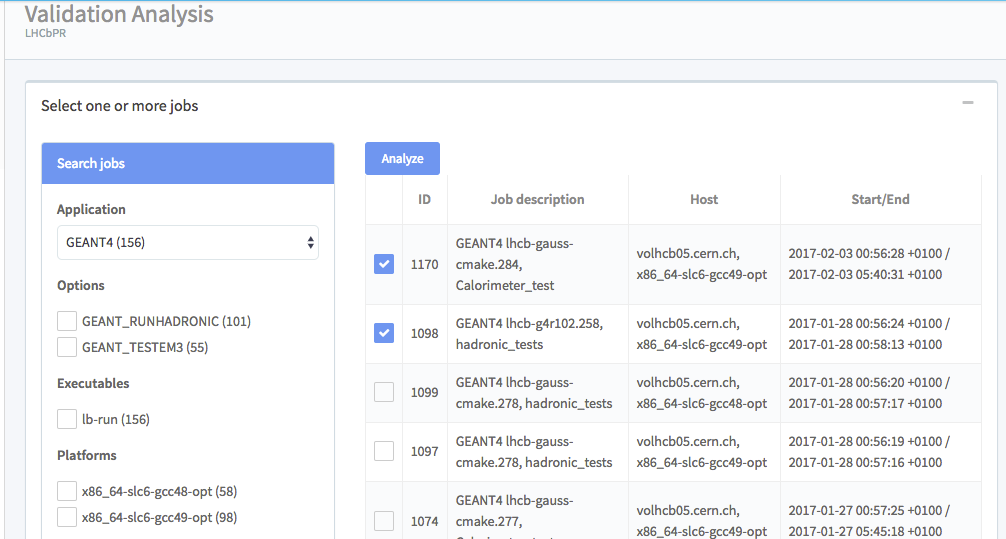
\includegraphics[width=0.6\textwidth,valign=t]{figs/webapp.png}}
  \label{fig:webapp:analyse}
}
\label{figwebapp}
\caption{Web application. Example of analysis module.}
\end{figure}

\section{Deployment}
The microservices pitfall appears to be the difficulty to develop components in different runtimes and in
different technology stacks.

For example, LHCbPR uses the following tools and libraries:
\begin{itemize}
\item \textbf{API service}. \textit{Django REST framework}~\cite{rest}, \textit{MySQL}
database, \textit{Gunicorn}~\cite{gunicorn} HTTP server
\item \textbf{ROOT service}. \textit{Flask}~\cite{flask} framework, \textit{Gunicorn} HTTP server, \textit{ROOT}.
\item \textbf{Web frontend}. \textit{NGINX}~\cite{nginx} HTTP server, \textit{Node.js}~\cite{node} for developing.
\end{itemize}

It will be hard for developers to test and deploy  such set of technologies
--- they need to be sure that services are run in the same environment, at
the same operating system and use the same versions of libraries. The most
challenging problem is to make all services to communicate with each other in the proper way.

These issues are resolved in LHCbPR by packaging services into
\textit{Docker~\cite{docker}} containers and orchestrating them with the \docker
\textit{Compose~\cite{compose}} tool. \docker containers guarantees that the
operating system and software will always run the same regardless of its
environemnt. \compose is a tool for defining and running multi-container \docker
applications. In our case such applications are LHCbPR's services. \composes
configuration can be shared between developers, so they can be sure that the
services communicate in the same environment. The deployment into production
becomes  smooth since the same
\docker images are used in development and production environments. The major difference
 between these environments is only \composes's configuration.

Figure~\ref{fig:nodes} shows the current deployment diagram of LHCbPR. At the
moment all services run at the dedicated virtual machine. All user requests go
through the proxy server that redirects them to the corresponding service. All
files, produced by tests, are stored at the network \textit{CEPH} volume which
is accesible from all serivices.
\textit{MySQL} database is managed by the CERN's \textit{Database On Demand} service.
Our plans is  to scale deployment to several virtual machines that can be done easy since
we can use \docker tools for that.  

\begin{figure}[H]
\begin{minipage}{\textwidth}
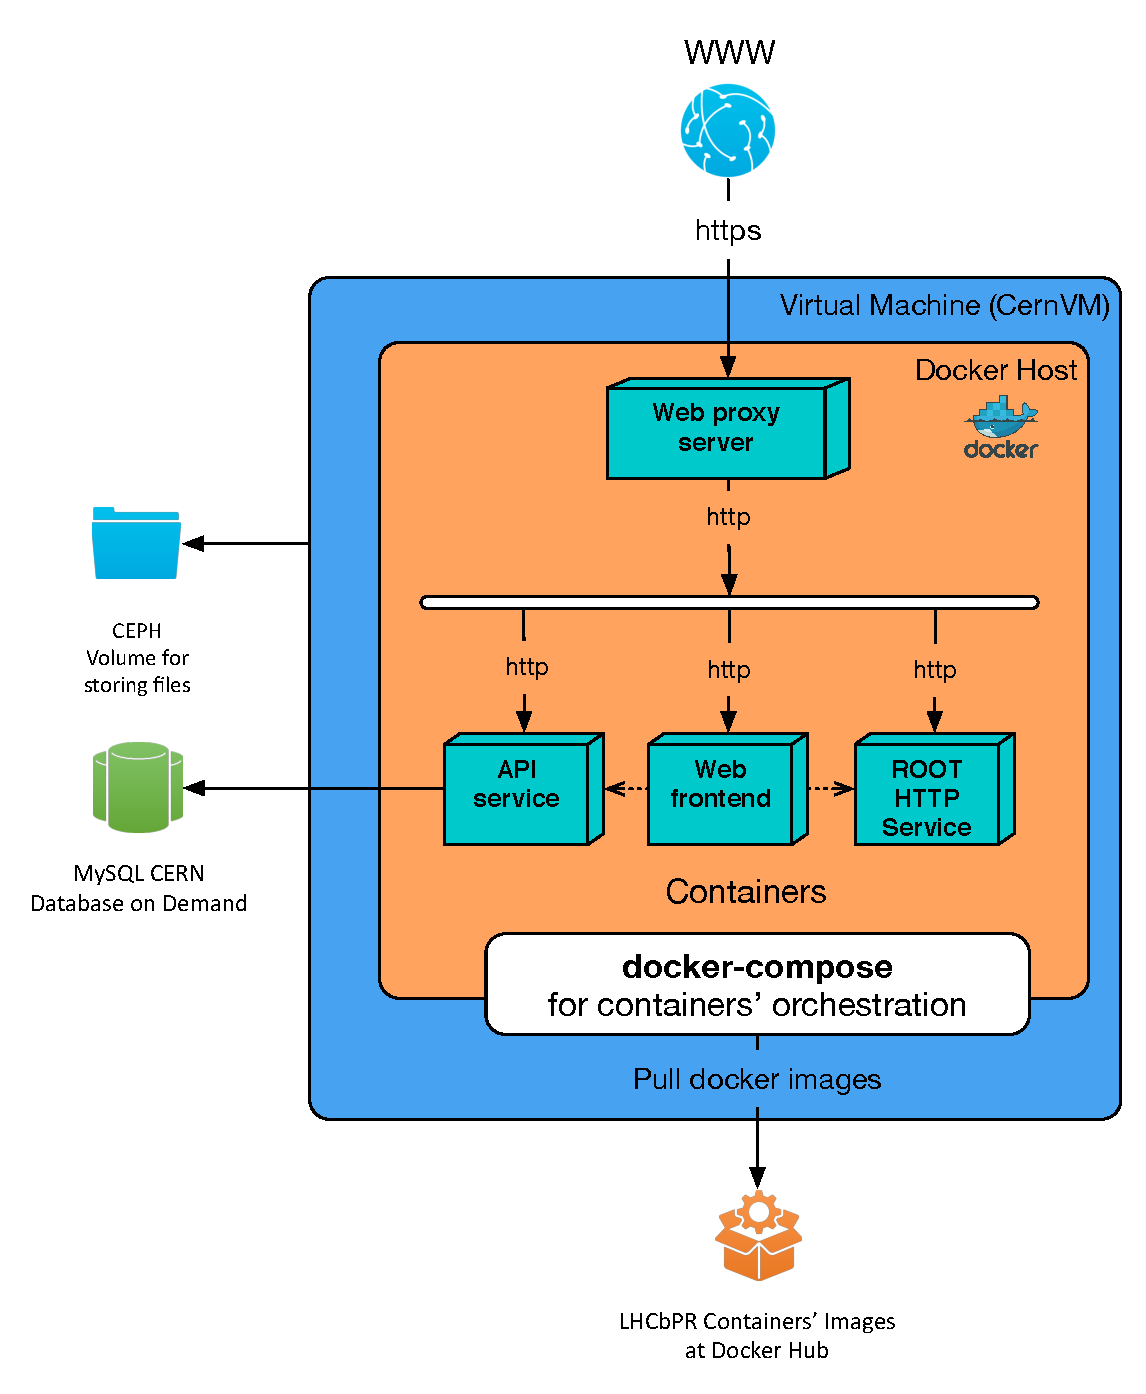
\includegraphics[width=0.75\textwidth]{figs/lhcbpr-nodes.pdf}
\caption{\label{fig:nodes}LHCbPR deployment diagram}
\end{minipage}
\end{figure}

\section{Summary}
In this paper we presented a new version of the LHCb performance and regression
testing framework. This versions demonstrates the advantages of microservices
approach for building complex applications.

The new LHCbPR is currently used in the production at LHCb experiment and handle
test results of simulation and trigger software. LHCbPR is not coupled with the
features specific to LHCb. It is possible to reuse LHCbPR in other experiments
or companies. For using LHCbPR, test services should only know how to retrieve
tests information from the LHCbPR API service and pack test results to the
format specific for this service.

We are currently focusing on improving generic analysis modules in LHCbPR web
application and always welcome any developers that would like to adopt LHCbPR
for their needs.


\section*{References}
\begin{thebibliography}{9}
\bibitem{lhcbpr} "Systematic profiling to monitor and specify the software refactoring process of the LHCb experiment", Ben
Couturier et al 2014 J. Phys.: Conf. Ser. 513 052020
\bibitem{lhcbsoft} "Software for the LHCb experiment", Corti, G. and Cattaneo, M. and Charpentier, P. and Frank,
M. and Koppenburg, P. and Mato, P. and Ranjard, F. and
Roiser, S. and Belyaev, I. and Barrand, G., 2006 IEEE
Trans. Nucl. Sci.
\bibitem{docker} Docker, https://www.docker.com/
\bibitem{compose} Docker Compose, https://docs.docker.com/compose/
\bibitem{rest} Django REST framework, http://www.django-rest-framework.org/
\bibitem{angular} AngularJS, https://angularjs.org/
\bibitem{gunicorn} Gunicorn, http://gunicorn.org/
\bibitem{nginx} NGINX, https://www.nginx.com/
\bibitem{node} Node.js, https://nodejs.org
\bibitem{flask} Flask, http://flask.pocoo.org/
% \bibitem{modular} "Modular Software Performance Monitoring",  Daniele Francesco Kruse and Karol Kruzelecki 2011 J. 
% Phys.: Conf. Ser. 331 042014. 
% \bibitem{gaudi} Barrand G et al. 2001 Comput. Phys. Commun. 140 45-55
% \bibitem{perfmon2} "Perfmon2: a standard performance monitoring interface for Linux", Stephane Eranian\\
% http://perfmon2.sourceforge.net/perfmon2-20080124.pdf
% \bibitem{vtune} \iamp \\ http://software.intel.com/en-us/articles/intel-vtune-amplifier-xe/
% \bibitem{perftools} \google Performance Tools \\ http://code.google.com/p/gperftools/
% \bibitem{reports} Custom pie chart reports \\ http://amazurov.ru/cern/hltprofilingresults/
% \bibitem{valgrind} Valgrind \\ http://valgrind.org/
\end{thebibliography}

\end{document}

